\problemname{Pipes}

Kazim\'ir got an important job at the plumbing department. He needs to connect certain pairs of locations by pipes. However, as the department's budget is very low, they have only two types of pipe parts: straight and ``elbow'' (L) shaped ones, all of the same size. Moreover, each pipe part is embedded into a square tile and the department provides a grid board onto which one can easily attach these tiles. The tiles can be rotated. The advantage of this design is that when two adjacent tiles' pipes align properly, there is no leaking. However, not having the option to go into the third dimension somewhat limits Kazim\'ir's connection options. Help him figure out whether he can connect the pairs of locations!

The grid board is of dimension $m\times n$. There are $\ell$ pairs of locations that need to be connected. Every location is along a side of the board, in the middle of a side of a grid square. Once Kazim\'ir places a pipe tile on a grid square, he is not allowed to place another tile on the same square.

\section*{Input}
The first line contains $k$, the number of input instances.
Each input instance is described on several lines. The first line contains three positive integers $m$, $n$, and $\ell$.
The second line contains $2\ell$ numbers $s_1,t_1,s_2,t_2,\dots,s_{\ell},t_{\ell}$ that describe the pairs of locations: Kazim\'ir needs to connect location $s_i$ to $t_i$ for every $i\in\{1,\dots,\ell\}$. The locations are described by numbers between 1 and $2(m+n)$, with 1 being the left side of the square in the top-left corner, then 2 is the left side of the square immediately below, 3 below that and so on, going in counterclockwise order around the boundary of the board; $2(m+n)$ is the top side of the top-left square. You may assume that $1\leq m\times n\leq$ 10,000 and that there are no duplicate locations -- all the $s_i$ and $t_j$ numbers are distinct.


\begin{figure}[h]
  \begin{center}
    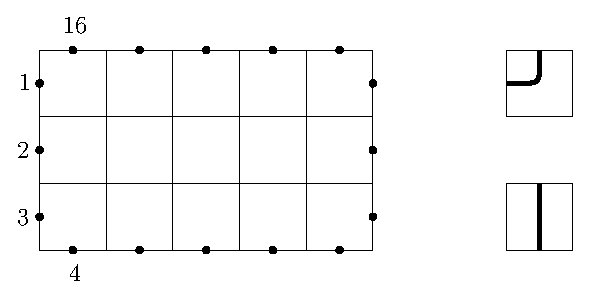
\includegraphics[scale=0.7]{pipe0}
  \end{center}
  \caption{Numbering of locations for an $m\times n = 3\times 5$ board. The types of tiles are shown on the right.}
\end{figure}

\section*{Output}
The output contains $k$ lines. The $i$-th line corresponds to the $i$-th input.
It contains {\tt YES} if it is possible to connect all the pairs of locations and {\tt NO} otherwise.

\section*{Note}
The three sample inputs are depicted below---sample input 1 on the left, with possible pipe connections between the locations; sample inputs 2 and 3 are in the middle and on the right, respectively.
\begin{figure}[h]
  \includegraphics[scale=0.7]{pipes1} \hfill
  \includegraphics[scale=0.7]{pipes2} \hfill
  \includegraphics[scale=0.7]{pipes3}
\end{figure}
